\documentclass[a4paper, 11pt]{article}
\usepackage[utf8]{inputenc}
\usepackage{hyperref}
\usepackage[margin=0.5in]{geometry}

\usepackage{amsmath}
\usepackage[arrowdel]{physics}
\usepackage{graphicx}
\usepackage{subfig}

\newcommand{\kb}{\ensuremath{k_{\text{B}}}}
\newcommand{\Na}{\ensuremath{N_{\text{A}}}}
\newcommand{\cc}[1]{#1^{\star}}
\newcommand{\adj}[1]{#1^{\dagger}}
\newcommand{\commut}[2]{[#1, #2]}
\newcommand{\cdir}[1]{\ensuremath{\left[#1\right]}}
\newcommand{\cplane}[1]{\ensuremath{\left(#1\right)}}
\newcommand{\cpset}[1]{\ensuremath{\left\{#1\right\}}}
\newcommand{\del}[3][]{\partial_{#2}^{#1}#3}
\newcommand{\deval}[4][]{\eval{\dv[#1]{#2}{#3}}_{#4}}
\newcommand{\pdeval}[4][]{\eval{\del[#1]{#2}{#3}}_{#4}}
\newcommand{\integ}[5][]{\int\limits_{#2}^{#3}\dd[#1]{#4}#5}

\title{Summary of SK2758 Solid State Physics}
\author{Yashar Honarmandi \\ yasharh@kth.se}
\date{\today}

\begin{document}

\maketitle

\begin{abstract}
	Denna sammanfattningen innehåller centrala definitioner och satser i SF1672 Flervariabelanalys.
\end{abstract}

\pagenumbering{roman}
\thispagestyle{empty}

\newpage

\tableofcontents

\newpage

\pagenumbering{arabic}

\section{Crystals}

\paragraph{Crystals}
Solid state physics, as we will study it, is concerned with crystals. A crystal is an arrangement of atoms which is repeated periodically. When developing the physics of crystals, we will assume their repetition to be infinite.

\paragraph{Basis}
The arrangement of atoms which is repeated in a crystal is termed the basis.

\paragraph{Lattices}
The set of points to which the basis is attached is termed the lattice.

\paragraph{Bravais Lattices}
A Bravais lattice is a lattice such that the arrangement of lattice points looks exactly equal from any lattice point. This turns out to be equivalent to the lattice being infinite and symmetric under certain discrete translations. We will treat crystal lattices as Bravais lattices.

The two-dimensional Bravais lattices are the rectangular,

\begin{figure}[!ht]
	\centering
	\subfloat[Square.]
	{
		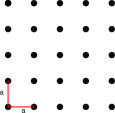
\includegraphics[width = 0.3\textwidth]{./Images/2d_square.pdf}
	}
	\hfil
	\subfloat[Rectangular.]
	{
		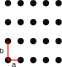
\includegraphics[width = 0.3\textwidth]{./Images/2d_rectangular.pdf}
	}
\end{figure}

%TODO: Add 2D and 3D Bravais lattices

\paragraph{Lattice Vectors}
The set $\{\vb{a}_{i}\}$ of lattice vectors of a Bravais lattice is the smallest possible set of vectors such that translating the lattice by $u_{i}\vb{a}_{i}$, where the $u_{i}$ are integers, leaves the lattice unchanged. There is an infinite number of ways to define the lattice vectors of a given lattice.

\paragraph{Primitive Lattice Vectors}
A set of lattice vectors is primitive if any two equivalent points are connected by integer combinations of the lattice vectors.

\paragraph{Crystal Axes}
The crystal axes are a set of directions that span space. These may be chosen according to, for instance, the primitive lattice vectors or other directions connected to the symmetry of the lattice.

\paragraph{Crystal Cell}
The crystal cell is the repeat unit of the crystal. It may be constructed in an infinite number of ways.

\paragraph{Lattice Constants}
Lattice constants are a set of parameters defining the dimensions of the cell.

\paragraph{Primitive Cell}
The primitive cell is a minimum-volume cell. It contains only one lattice point, and is thus termed a unit cell. Its infinite translation throughout space yields the lattice.

\paragraph{Primitive Basis}
The primitive basis is the basis associated with the primitive cell.

\paragraph{Wigner-Seitz Cell}
The Wigner-Seitz Cell is the cell constructed by for any lattice point dividing space into two at the middle of and normal to the line between the point in question and all other points, and choosing the smallest possible region of space containing the point from this.

\paragraph{Lattice Point Group}
The lattice point group is the group of operations which, applied about a lattice point (i.e. keeping this point fixed), leaves the lattice unchanged. Examples of possible fundamental operations include:
\begin{itemize}
	\item rotations.
	\item reflections.
\end{itemize}

\paragraph{Lattice Space Group}
The space group of the Bravais lattices is the group of symmetries of all Bravais lattices of a given dimensionality. It contains both point groups and translations.

\paragraph{$n$-Fold Rotations}
An $n$-fold rotation is a rotation operation such that it reduces to the identity operation when applied $n$ times. Lattices cannot be symmetric under $5$-fold rotation.

\paragraph{Crystal Planes}
In a cell it is useful to define crystallographic planes. These are indicated by a set of indices \cplane{hkl}, the computation of which we will return to. A bar above any element indicates that element to be negative.

A set of parallel planes such that all lattice points are contained in the set may be denoted \cpset{hkl}.

\paragraph{Crystallographic Directions}
Likewise we define crystallographic directions by the notation \cdir{uvw}. The indices are the set of the smallest integers such that they form a vector parallel to the one in question.

\paragraph{Random Stacking}
Randomly stacked crystals are formed by densely packed layers of atoms being stacked without long-range order in the stacking direction.

\paragraph{Polytopism}
Polytopism is a milder variation of random stacking, where the order of the stacked layers is extremely long-range.

%TODO: Add special structures

\paragraph{X-Ray Diffraction}
X-ray diffraction is the process of shining X-rays onto a material in order to characterize it. Before atomic physics, it was discovered that solids scattered X-rays intensely in specific directions, as opposed to light, which was reflected by the solid. In the context of solid-state physics, we can interpret this as crystal planes acting as diffraction grids that scatter the X-rays. This interpretation makes sense because the wavelength of X-rays is comparable to interatomic distances in a solid, consistent with the regime in which classical wave physics predicts that diffraction phenomena are significant, and the scattered light being localized is consistent with diffraction of other waves.

\paragraph{Bragg's Law}
Bragg's law was a first attempt at explaining X-ray diffraction patterns. To derive it, consider a solid composed of aligned and stacked atomic planes separated by a distance $d$ on which electromagnetic radiation of wavelength $\lambda$ is incident at angle $\theta$ to the planes, and suppose each plane reflects the radiation specularly (following the law of reflection) and elastically (preserving the wavelength). Comparing radiation reflected from two adjacent layers, the light in the lower layer travels a distance $2d\sin{\theta}$ longer. In order for the radiation from these layers to interfere constructively, we must have
\begin{align*}
	2d\sin{\theta} = n\lambda,\ n = 1, 2, \dots
\end{align*}
This is Bragg's law. It is a very rough description of X-ray diffraction, but predicts the phenomenology correctly. It also predicts that diffraction occurs for $\lambda < 2d$, which is why light, for instance, is not diffracted by solids.

\paragraph{Fourier Analysis and Reciprocal Space}
The translational symmetry of the lattice implies that the tools of Fourier analysis are applicable when studying solid-state physics. Any observable $A$ defined on the crystal lattice may be written as
\begin{align*}
	A = \sum\limits_{\vb{G}}A_{\vb{G}}e^{i\vb{G}\cdot\vb{r}}.
\end{align*}
The coefficients in the series expansion are given by
\begin{align*}
	A_{\vb{G}} = \frac{1}{V_{\text{cell}}}\integ[d]{\text{cell}}{}{\vb{r}}{A(\vb{r})e^{-i\vb{G}\cdot\vb{r}}}.
\end{align*}
In order for $A$ to be an observable, we must have $A_{-\vb{G}} = \cc{A_{\vb{G}}}$. The fact that $A$ is an observable on the crystal lattice implies that it must have the same symmetries - in particular translational symmetry. This implies
\begin{align*}
	A(\vb{r} + u_{i}\vb{a}_{i}) = A(\vb{r}) \implies u_{i}\vb{G}\cdot\vb{a}_{i} = 2\pi n
\end{align*}
where $n$ is an integer. The vectors $\vb{G}$ must have reciprocal length as their dimension, and are thus vectors in what is termed reciprocal space.

\paragraph{The Reciprocal Lattice}
The simplest choice of vectors satisfying
\begin{align*}
	u_{i}\vb{G}\cdot\vb{a}_{i} = 2\pi n
\end{align*}
is integer combinations of a set of vectors $\{\vb{b}_{i}\}$ such that $\vb{a}_{i}\cdot\vb{b}_{j} = 2\pi\delta_{ij}$. The set of vectors $\{\vb{b}_{i}\}$ thus defines a Bravais lattice in reciprocal space, termed the reciprocal lattice. In three dimensions, the explicit formula for the reciprocal lattice vectors is
\begin{align*}
	\vb{b}_{1} = \frac{2\pi}{V_{\text{cell}}}\vb{a}_{2}\times\vb{a}_{3},\ V_{\text{cell}} = \vb{a}_{1}\cdot(\vb{a}_{2}\times\vb{a}_{3})
\end{align*}
with cyclic permutation of the indices yielding the other two.

\paragraph{Crystal Planes and the Reciprocal Lattice}
Assume that there is a lattice point in the origin and that the closest crystal plane with orientation specified by the normal vector $\vb{n}$ is a distance $d$ from the origin. Any plane parallel to the plane in question is described by
\begin{align*}
	\vb{r}\cdot\vb{n} = md,\ m = 0, \pm 1, \dots
\end{align*}

Consider now a translation by $\vb{T}$ such that the lattice is left invariant. Assuming the translation to be between lattice points, the translation must satisfy the equation of some crystal plane, implying
\begin{align*}
	\vb{T}\cdot\vb{n} = md.
\end{align*}
In particular, if the translation is to a point in a plane adjacent to the origin, we have
\begin{align*}
	\vb{T}\cdot\frac{2\pi}{d}\vb{n} = 2\pi.
\end{align*}
Comparing this to the definition of the reciprocal lattice implies that the plane is normal to a reciprocal lattice vector
\begin{align*}
	\vb{G} = \frac{2\pi}{d}\vb{n}.
\end{align*}
This is the shortest reciprocal lattice vector describing the plane. The expression above implies
\begin{align*}
	d = \frac{2\pi}{\abs{\vb{G}}}.
\end{align*}

\paragraph{Miller Indices}
Returning to the indexing system for crystal planes, we may decompose the normal vector as
\begin{align*}
	\vb{G} = h\vb{b}_{1} + k\vb{b}_{2} + l\vb{b}_{3}.
\end{align*}
These indices are exactly the indices used to describe a crystal plane, and are termed Miller indices. As $\vb{G}$ is the shortest vector describing the plane, the indices cannot contain any common factors.

The Miller indices may also be computed from the real lattice according to the following rules:
\begin{enumerate}
	\item For each axis, defined by the lattice vectors, identify the intercepts of the plane with the axis as units of the lattice parameters.
	\item Compute the reciprocals of each intercept.
	\item Reduce to three integers with the same ratio.
\end{enumerate}

\paragraph{Interplanar Distances}
Consider the set of \cpset{hkl} planes. We are interested in computing the distance between two adjacent such planes. To do this, we will first need a unit normal to any such plane. According to the construction of the Miller indices, the vectors
\begin{align*}
\vb{v}_{1} = \frac{1}{h}\vb{a}_{1} - \frac{1}{k}\vb{a}_{2},\ \vb{v}_{2} = \frac{1}{h}\vb{a}_{1} - \frac{1}{l}\vb{a}_{3}
\end{align*}
span the plane, apart from some constant spatial shift. Hence we are interested in a vector that is simultaneously normal to both of these. One possible choice is
\begin{align*}
	\vb{G}_{hkl} = h\vb{b}_{1} + k\vb{b}_{2} + l\vb{b}_{3}.
\end{align*}
From this, obtaining a unit normal is trivial. Next we need a vector from one plane to the other. One possible choice is
\begin{align*}
	\vb{T} = \frac{1}{h}\vb{a}_{1},
\end{align*}
as one cell has space for $h$ planes of this type when counted along the $\vb{a}_{1}$ direction. From this, the distance is given by
\begin{align*}
	d = \frac{1}{\abs{\vb{G}_{hkl}}}\vb{G}_{hkl}\cdot\vb{T} = \frac{2\pi}{\abs{\vb{G}_{hkl}}},
\end{align*}
which is true for any Bravais lattice.

\paragraph{Diffraction by Solids}
Using the language of Fourier analysis and reciprocal space, we will try to derive a more sophisticated diffraction condition.

To do this, consider a crystal exposed to far-field radiation described by a wave vector $\vb{k}$ which is scattered elastically by the crystal in an arbitrary direction and observed in the far-field region in some direction, in which the wave vector is $\vb{k}^{\prime}$. Considering the interference between two points displaced by $\vb{r}$, the phase difference between the radiation from the two points is $(\vb{k} - \vb{k}^{\prime})\cdot\vb{r}$. Supposing that the amplitude of the scattered wave is proportional to the electron density (or, really, any property defined on the lattice), the total scattered amplitude is proportional to the (confusingly termed) scattering amplitude
\begin{align*}
	F = \integ[d]{}{}{\vb{r}}{n(\vb{r})e^{i(\vb{k} - \vb{k}^{\prime})\cdot\vb{r}}}.
\end{align*}
Adding the series expansion of the electron density yields
\begin{align*}
	F = \integ[d]{}{}{\vb{r}}{\sum\limits_{\vb{G}}n_{\vb{G}}e^{i\vb{G}\cdot\vb{r}}e^{-i\Delta\vb{k}\cdot\vb{r}}} = \integ[d]{}{}{\vb{r}}{\sum\limits_{\vb{G}}n_{\vb{G}}e^{i(\vb{G} - \Delta\vb{k})\cdot\vb{r}}} = \sum\limits_{\vb{G}}\integ[d]{}{}{\vb{r}}{n_{\vb{G}}e^{i(\vb{G} - \Delta\vb{k})\cdot\vb{r}}}.
\end{align*}
For the case $\Delta\vb{k} = \vb{G}$ for any one particular reciprocal lattice vector, the exponential in this term vanishes, leaving a term $Vn_{\vb{G}}$. It can be shown that all other terms in the scattering amplitude vanish, yielding $F = Vn_{\vb{G}}$ for this case and $F = 0$ otherwise. The most fundamental diffraction condition is thus
\begin{align*}
	\Delta\vb{k} = \vb{G}.
\end{align*}

While we have in principle obtained a diffraction condition now, we can simplify it by using the fact that the scattering is inelastic. We obtain
\begin{align*}
	2\vb{k}\cdot\vb{G} + G^{2} = 0.
\end{align*}
It may be rewritten by swapping $\vb{G}$ for $-\vb{G}$, which is also a reciprocal lattice vector, to yield
\begin{align*}
	2\vb{k}\cdot\vb{G} = G^{2}.
\end{align*}

Note that this implies that information about the reciprocal lattice, and therefore the lattice itself, may be obtained from diffraction experiments.

\paragraph{Laue's Equations}
The fundamental diffraction criterion implies
\begin{align*}
	\Delta\vb{k}\cdot\vb{a}_{i} = 2\pi v_{i}
\end{align*}
for some integer $v_{i}$, simultaneously for all lattive vectors. This implies that reflections are only found at the intersection of three cones in reciprocal space. This is very strict, and such reflections must be found by sweeping in crystal orientation and/or wavelength or by chance.

\paragraph{The Ewald Sphere}
The Ewald sphere is a tool for visualizing the necessary conditions for diffractions. To construct it, draw the incident wave vector starting in a point such that it terminates in a reciprocal lattice point. From the starting point, draw a sphere of radius $k$. All reciprocal lattice points corresponding to a diffraction peak are found on this sphere.

\paragraph{Brillouin Zones}
To introduce the concept of Brillouin zones, rewrite the diffraction condition as
\begin{align*}
	\vb{k}\cdot\frac{1}{2}\vb{G} = \left(\frac{1}{2}G\right)^{2}.
\end{align*}
For a fixed $\vb{G}$, this equation defines the set of wave vectors terminating on the bisector of $\vb{G}$. This is similar to the construction of the Wigner-Seitz cell in real space, but now extended to construct zones using all points in the reciprocal lattice. Constructing these bisectors divides the reciprocal space into Brillouin zones (a single Brillouin zone is the combinations of all zones a fixed number of zones from the central zone). The central zone, which is the Wigner-Seitz cell in reciprocal space, is the first Brillouin zone.

\paragraph{Volume of the Brillouin Zone}
We would like to compute the volume of the Brillouin zone in terms of the volume of the unit cell. To do this, we note that the unit cell volume is given by
\begin{align*}
	V_{\text{c}} = \vb{a}_{1}\cdot(\vb{a}_{2}\times\vb{a}_{3}).
\end{align*}
Using this, the volume of the Brillouin zone is given by
\begin{align*}
	V_{\text{r}} = \vb{b}_{1}\cdot(\vb{b}_{2}\times\vb{b}_{3}).
\end{align*}
The vector in the parenthesis is given by
\begin{align*}
	\vb{b}_{2}\times\vb{b}_{3} &= \frac{(2\pi)^{2}}{V_{\text{c}}^{2}}(\vb{a}_{3}\times\vb{a}_{1})\times (\vb{a}_{1}\times\vb{a}_{2}) \\
	                           &= \frac{(2\pi)^{2}}{V_{\text{c}}^{2}}((\vb{a}_{3}\cdot(\vb{a}_{1}\times\vb{a}_{2}))\vb{a}_{1} - (\vb{a}_{3}\cdot(\vb{a}_{1}\times\vb{a}_{1}))\vb{a}_{2}) \\
	                           &= \frac{(2\pi)^{2}}{V_{\text{c}}}\vb{a}_{1},
\end{align*}
and thus the volume of the Brillouin zone is given by
\begin{align*}
	V_{\text{r}} = \frac{(2\pi)^{3}}{V_{\text{c}}}.
\end{align*}

\paragraph{The Structure Factor and Atomic Form Factor}
The diffraction condition is stated in terms of reciprocal lattice vectors obtained from the primitive lattice vectors. However, especially in experimental contexts, the primitive unit cell is not the geometry of choice for studying materials. Instead, one can use inherent ambiguities in choices of repeat units of the crystal to study geometries with, for instance, more or simpler symmetries. When considering such geometries, the diffraction conditions is only necessary, not sufficient. We will now study diffraction for such cases.

Consider a crystal built up of some kind of cell, not necessarily a primitive one. When the diffraction condition is satisfied, i.e. $\Delta\vb{k} = \vb{G}$ for some reciprocal lattice vector corresponding to the chosen cell, the scattering amplitude for a crystal of $N$ cells becomes
\begin{align*}
	F = \integ[d]{}{}{\vb{r}}{n(\vb{r})e^{-i\vb{G}\cdot\vb{r}}} = N\integ[d]{\text{cell}}{}{\vb{r}}{n(\vb{r})e^{-i\vb{G}\cdot\vb{r}}} = NS_{\vb{G}},
\end{align*}
where we have introduced the structure factor $S_{\vb{G}}$, which describes the effect of the electron distribution in the cell on the scattering amplitude for a given diffraction peak.

Writing the electron density as a superposition of contributions from each atom in the basis (this decomposition is not unique, but somehow this is not a problem), we obtain
\begin{align*}
	S_{\vb{G}} = \integ[d]{\text{cell}}{}{\vb{r}}{\sum n_{j}(\vb{r} - \vb{r}_{j})e^{-i\vb{G}\cdot\vb{r}}}
\end{align*}
where the $\vb{r}_{j}$ are the positions of the atoms in the basis. We rewrite this as
\begin{align*}
	S_{\vb{G}} = \sum\integ[d]{\text{cell}}{}{\vb{r}}{n_{j}(\vb{r} - \vb{r}_{j})e^{-i\vb{G}\cdot\vb{r}}} = \sum e^{-i\vb{G}\cdot\vb{r}_{j}}\integ[d]{\text{cell}}{}{\vb{r}}{n_{j}(\vb{r})e^{-i\vb{G}\cdot\vb{r}}}.
\end{align*}
Defining the atomic form factor
\begin{align*}
	f_{j, \vb{G}} = \integ[d]{\text{cell}}{}{\vb{r}}{n_{j}(\vb{r})e^{-i\vb{G}\cdot\vb{r}}}
\end{align*}
we have
\begin{align*}
	S_{\vb{G}} = \sum f_{j, \vb{G}}e^{-i\vb{G}\cdot\vb{r}_{j}}.
\end{align*}
The requirement for diffraction is thus that $\Delta\vb{k} = \vb{G}$ and the structure factor being non-zero.

When observing electron distributions in solids, these appear close to those of free atoms. This does not mean that electrons are not distributed in a solid versus for free atoms, but that these corrections do not have a major effect on the atomic form factors. Thus it may be relevant to write these as
\begin{align*}
	f_{j, \vb{G}} = \integ[d]{}{}{\vb{r}}{n_{j}(\vb{r})e^{-i\vb{G}\cdot\vb{r}}}
\end{align*}
where the electron distribution is that of a free atom and the integration is performed over all of space.

The astute reader might have noticed that when considering the primitive unit cell of a crystal with one atom in the basis, the structure factor is trivial. One could thus ask whether this was really necessary. The answer to the latter question is left to experimentalists, but I can confirm that this derivation neither adds nor subtracts to our knowledge. If you have chosen the primitive cell, the structure factor is trivial and diffraction occurs for every observation such that the diffraction criterion is satisfied. For other choices of cells, certain reciprocal lattice vectors will produce a structure factor equal to zero. This is because these do not correspond to reciprocal lattice vectors of the primitive cell. Someone should prove this more rigorously. Can we be sure that other choices of cells cover all possible reciprocal lattice vectors of the primitive cell? Yes, as non-primitive cells must have longer lattice vectors, corresponding to shorter reciprocal lattice vectors, implying that the reciprocal lattice vectors of the primitive cell should be possible to express as combinations of the reciprocal lattice vectors of the non-primitive cell.

\paragraph{Cohesive Energy}
The cohesive energy of a crystal is the energy required to separate the crystal into neutral free atoms at rest at infinite separation.

\paragraph{Types of Crystal Binding}
The different types of crystal binding and their origins are
\begin{itemize}
	\item van der Waals binding, which occurs due to fluctuating electric dipoles in atoms and molecules.
	\item ionic binding, which occurs due to Coulomb forces between ions.
	\item covalent binding, which occurs due to the filling of electron states localized between atoms.
	\item metal binding, where valence electrons form a gas throughout the crystal and balance repulsion between the metal atoms in the lattice.
\end{itemize}

\paragraph{van der Waals Energy}
%TODO: Derivation of van der Waals energy
The van der Waals interaction between two atoms in a crystal or molecule is modelled as a potential of the form
\begin{align*}
	V = 4\varepsilon\left(\left(\frac{\sigma}{R}\right)^{12} - \left(\frac{\sigma}{R}\right)^{6}\right)
\end{align*}
with a positive term from Pauli repulsion and a negative term from attraction between fluctuating dipoles.

For a crystal of $N$ atoms the cohesive energy due to van der Waals interaction becomes
\begin{align*}
	U = 2N\varepsilon\left(\sum\limits_{j}\left(\frac{\sigma}{R_{j}}\right)^{12} - \left(\frac{\sigma}{R_{j}}\right)^{6}\right).
\end{align*}
Re-expressing this in terms of nearest-neighbour distances $R$ in the lattice, we can write $R_{j} = p_{j}R$ to obtain
\begin{align*}
	U = 2N\varepsilon\left(\left(\frac{\sigma}{R}\right)^{12}\sum\limits_{j}\frac{1}{p_{j}^{12}} - \left(\frac{\sigma}{R}\right)^{6}\sum\limits_{j}\frac{1}{p_{j}^{6}}\right)
\end{align*}
where we have divided by two in order to distribute the interaction energy evenly between the atoms. The two summations are determined solely by the crystal structure.

\paragraph{Ionic Binding}
Ionic interactions between two atoms in a crystal is modelled as a potential of the form
\begin{align*}
	V = \lambda e^{-\frac{R_{ij}}{\rho}} \pm \frac{q^{2}}{4\pi\varepsilon_{0}R_{ij}}
\end{align*}
with a positive term from Pauli repulsion and a negative term from attraction between charged particles. The Pauli term is typically only included for nearest neighbours.

For a crystal of $N$ atoms the cohesive energy due to ionic interaction becoms
\begin{align*}
	U = N\left(Z\lambda e^{-\frac{R}{\rho}} + \sum\limits_{j}(-1)^{g(j)}\frac{q^{2}}{4\pi\varepsilon_{0}R_{j}}\right)
\end{align*}
where we have introduced the nearest-neighbour distance $R$ and the function $g$ describing whether atom  $j$ has an equal or opposite charge to that of the atom in the origin. Re-expressing the Coulomb term in terms of nearest-neighbour distances we obtain
\begin{align*}
	U = N\left(Z\lambda e^{-\frac{R}{\rho}} - \alpha\frac{q^{2}}{4\pi\varepsilon_{0}R_{ij}}\right)
\end{align*}
where $Z$ is the coordination number of a given ion and
\begin{align*}
	\alpha = \sum\limits\frac{(-1)^{g(j)}}{p_{j}}
\end{align*}
is termed the Madelung constant and depends only on the crystal structure.

\paragraph{Covalently Bound Solids}
Solids bound by covalent force have localized electrons due to the nature of the bonds in the solid, meaning that such bonds are typically found in insulators and semiconductors.

\paragraph{Metals}
Electrons in metals move around in a gas, hence metals are generally good conductors.

\paragraph{Atomic Radii}
The introduced parameters in the interaction potentials described above that have dimensions of length are essentially dependent on atomic radii. It turns out that atomic radii are largely independent of the composition of the material in which any given atom is found. However, they are significantly affected by coordination number.

\section{Phonons and Crystal Vibration}

\paragraph{The Monoatomic Chain}
Vibrations in a crystal lattice along a certain crystal direction are vibrations along a chain of atoms lying in that direction. Hence we will need to understand the (classical) physics of particles on chains.

%TODO: Show without assuming x dependence
Consider a chain of atoms at positions $x_{n} = na + u_{n}$, the first term of which is the equliibrium position and the second is the fluctuations from equilibrium. Assuming a harmonic potential with intensity $C$ between nearest neighbours in the chain, your favorite choice of equations of motion will yield
\begin{align*}
	m\dv[2]{x_{n}}{t} = m\dv[2]{u_{n}}{t} = C(x_{n + 1} - x_{n}) - C(x_{n} - x_{n - 1}) = C(x_{n + 1} + x_{n - 1} - 2x_{n}) = C(u_{n + 1} + u_{n - 1} - 2u_{n}).
\end{align*}
When studying lattice vibrations, we are interested in solutions to the equations of motion which are travelling waves, of the form
\begin{align*}
	u_{n} = u_{0}e^{i(Kna - \omega t)}.
\end{align*}
Inserting this into the equations of motion yields
\begin{align*}
	-m\omega^{2}u_{0}e^{i(Kna - \omega t)} = Cu_{0}e^{i(Kna - \omega t)}\left(e^{iKa} + e^{-iKa} - 2\right) = 2Cu_{0}e^{i(Kna - \omega t)}\left(\cos{Ka} - 1\right) = -4Cu_{0}e^{i(Kna - \omega t)}\sin[2](\frac{Ka}{2}).
\end{align*}
This implies the dispersion relation
\begin{align*}
	\omega = \sqrt{\frac{4C}{m}}\abs{\sin(\frac{Ka}{2})}.
\end{align*}

To continue our study, we introduce
\begin{align*}
	\xi = \frac{Ka}{2\pi},\ \omega_{0} = \sqrt{\frac{4C}{m}},
\end{align*}
allowing us to write the dispersion relation as
\begin{align*}
	\omega = \omega_{0}\abs{\sin(\pi\xi)}.
\end{align*}
Firstly we note that the dispersion relation has a period of $\pi$ in the new coordinates. In addition, we note that $\xi$ for this chain is a measure of progression in the reciprocal lattice - each integer value of $\xi$ corresponds to a reciprocal lattice point. This means that all of the physics of the chain are contained within the interval $-\frac{1}{2} < \xi < \frac{1}{2}$, which is the first Brillouin zone of the lattice.

The periodicity of the dispersion relation has an interpretation. Suppose that $K = k + \frac{2\pi}{a}$ where $k$ is within the first Brillouin zone. The motion of any particle in the chain when exposed to such a wave is given by
\begin{align*}
	u_{n} = u_{0}e^{i(Kna - \omega t)} = u_{0}e^{2\pi ni}e^{i\left(kna - \omega t\right)} = u_{0}e^{i\left(kna - \omega t\right)}.
\end{align*}
Hence the periodicity of the dispersion relation is due to the fact that the travelling wave is only defined at discrete points.

The group velocity of such lattice vibrations is given by
\begin{align*}
	v_{\text{g}} = \dv{\omega}{K} = \frac{1}{2\omega}\dv{\omega^{2}}{K} = \frac{1}{2\omega_{0}\abs{\sin(\pi\xi)}}\cdot \frac{2a\omega_{0}^{2}}{2}\sin(\frac{Ka}{2})\cos(\frac{Ka}{2}) = \frac{1}{2}a\omega_{0}\cos(\pi\xi)\text{sgn}\left(\sin(\pi\xi)\right),
\end{align*}
where the last factor merely describes the direction of propagation. In the long-wavelength limit, close to the origin in reciprocal space, we obtain
\begin{align*}
	\omega \approx \omega_{0}\pi\xi = \frac{1}{2}Ka\omega_{0},\ v_{\text{g}} \approx \frac{1}{2}a\omega_{0},
\end{align*}
implying the linear dispersion relation $\omega = v_{\text{g}}K$. Identifying $Ca$ as a measure of the tension and $\frac{m}{a}$ as the density, we also have
\begin{align*}
	v_{\text{g}} = \sqrt{\frac{T}{\rho}},
\end{align*}
as expected for acoustic waves in a solid. When approaching the Brillouin zone boundary, we obtain
\begin{align*}
	v_{\text{g}} = 0,
\end{align*}
representing a standing wave solution. The wavelength corresponding to the zone boundary is the shortest wavelength that can propagate in the material.

\paragraph{The Diatomic Chain}
To study the effect of the basis, consider a chain of atoms with two atoms in the basis and lattice parameter $a$. Denoting the fluctuations of each type of atom by $u$ and $v$ respectively and only considering nearest-neighbour interactions, the equations of motion are
\begin{align*}
	m_{1}\dv[2]{u_{n}}{t} = C(v_{n} + v_{n - 1} - 2u_{n}),\ m_{2}\dv[2]{v_{n}}{t} = C(u_{n + 1} + u_{n} - 2v_{n}).
\end{align*}
We again look for plane wave solutions of the form
\begin{align*}
	u_{n} = u_{0}e^{i(Kna - \omega t)},\ v_{n} = v_{0}e^{i(Kna - \omega t)}.
\end{align*}
Inserting this into the equations of motion yields
\begin{align*}
	-m_{1}\omega^{2}u_{0}e^{i(Kna - \omega t)} &= C\left(v_{0}e^{i(Kna - \omega t)} + v_{0}e^{i(K(n - 1)a - \omega t)} - 2u_{0}e^{i(Kna - \omega t)}\right) \\
	                                           &= Ce^{-i(Kna - \omega t)}\left(v_{0}\left(1 + e^{-iKa}\right) - 2u_{0}\right), \\
	-m_{2}\omega^{2}v_{0}e^{i(Kna - \omega t)} &= C\left(u_{0}e^{i(K(n + 1)a - \omega t)} + u_{0}e^{i(Kna - \omega t)} - 2v_{0}e^{i(Kna - \omega t)}\right) \\
	                                           &= Ce^{i(Kna - \omega t)}\left(u_{0}\left(e^{iKa} + 1\right) - 2v_{0}\right).
\end{align*}
This is a homogenous system of equations in the amplitudes. A non-trivial solution (corresponding to there being motion in the system) corresponds to the determinant of the coefficient matrix being zero. This implies
\begin{align*}
	\mqty
	[
		2C - m_{1}\omega^{2}       & -C\left(1 + e^{-iKa}\right) \\
		-C\left(e^{iKa} + 1\right) & 2C - m_{2}\omega^{2}
	]
	&= 0, \\
	(2C - m_{1}\omega^{2})(2C - m_{2}\omega^{2}) - C^{2}\left(1 + e^{-iKa}\right)\left(e^{iKa} + 1\right) &= 0, \\
	m_{1}m_{2}\omega^{4} - 2C(m_{1} + m_{2})\omega^{2} + 2C^{2}\left(1 - \cos(Ka)\right) &= 0,
\end{align*}
with solution
\begin{align*}
	\omega^{2} &= \frac{2C(m_{1} + m_{2}) \pm \sqrt{4C^{2}(m_{1} + m_{2})^{2} - 8m_{1}m_{2}C^{2}\left(1 - \cos(Ka)\right)}}{2m_{1}m_{2}}.
\end{align*}
Defining
\begin{align*}
	\omega_{0} = \sqrt{\frac{C(m_{1} + m_{2})}{m_{1}m_{2}}}
\end{align*}
we obtain
\begin{align*}
	\omega^{2} &= \omega_{0}^{2}\left(1 \pm \sqrt{1 - 4\frac{m_{1}m_{2}}{(m_{1} + m_{2})^{2}}\sin[2](\frac{1}{2}Ka)}\right).
\end{align*}
The two choices of sign here represent two so-called branches of the dispersion relation, one termed the optical branch and the other the acoustic branch. The terminology will be clarified later.

We proceed by studying the limiting cases. In the low-wavelength limit we have
\begin{align*}
	\omega^{2} &\approx \omega_{0}^{2}\left(1 \pm \sqrt{1 - \frac{m_{1}m_{2}}{(m_{1} + m_{2})^{2}}(Ka)^{2}}\right) \\
	           &\approx \omega_{0}^{2}\left(1 \pm 1 \mp \frac{m_{1}m_{2}}{2(m_{1} + m_{2})^{2}}(Ka)^{2}\right),
\end{align*}
yielding
\begin{align*}
	\omega_{\text{op}} \approx \sqrt{2}\omega_{0},\ \omega_{\text{ac}} \approx \frac{\sqrt{C}}{\sqrt{2(m_{1} + m_{2})}}\abs{Ka}.
\end{align*}
For the optical branch, we thus obtain
\begin{align*}
	\frac{u_{0}}{v_{0}} = \frac{2C}{2C - 2m_{1}\omega_{0}^{2}} = \frac{2m_{2}}{2m_{2} - 2(m_{1} + m_{2})} = -\frac{m_{2}}{m_{1}},
\end{align*}
and for the acoustic branch we obtain
\begin{align*}
	\frac{u_{0}}{v_{0}} = \frac{2C}{2C - 2m_{1}\frac{C}{2(m_{1} + m_{2})}(Ka)^{2}} \approx 1,
\end{align*}
This reveals the nature of the nomenclature, as acoustic modes correspond to atoms oscillating in phase and propagating acoustic waves, whereas optical modes correspond to atoms being in anti-phase and can thus be excited by electromagnetic waves in ionic crystals.

Simultaneously plotting the dispersion relations of the two branches in the first Brillouin zone yields two different curves. As the anti-phase solution in the low-wavelength limit for the optical branch corresponds to a periodicity of $\lambda = a$ for the motion, we can interpret excitations of oscillations in the chain as starting in the acoustic branch for small $K$ and following this dispersion relation before moving into the optical branch when crossing the Brillouin zone boundary. This transition is not smooth, as at the Brillouin zone boundary we have
\begin{align*}
	\omega^{2} &= \omega_{0}^{2}\left(1 \pm \sqrt{1 - 4\frac{m_{1}m_{2}}{(m_{1} + m_{2})^{2}}}\right) \\
	           &= \frac{\omega_{0}^{2}}{m_{1} + m_{2}}\left(m_{1} + m_{2} \pm \sqrt{(m_{1} + m_{2})^{2} - 4m_{1}m_{2}}\right) \\
	           &= \frac{C}{m_{1}m_{2}}\left(m_{1} + m_{2} \pm (m_{1} - m_{2})\right),
\end{align*}
assuming $m_{1} > m_{2}$, with permuting the indices yielding the other result. Specifically, for the two branches we obtain
\begin{align*}
	\omega_{\text{op}} = \sqrt{\frac{2C}{m_{2}}},\ \omega_{\text{ac}} = \sqrt{\frac{2C}{m_{1}}},
\end{align*}
and frequencies between these two cannot be excited in the chain. This gap must thus be crossed in order for the described excitation to occur. Furthermore, as each of these frequencies correspond (I think) to the harmonic oscillation frequencies of only one sort of atom in the harmonic potential created by the static nearest neighbours, we can interpret it as each branch approaching a state where only one kind of atom is excited, and the frequency gap is due to the different masses of the atoms.

\paragraph{Crystal Vibrations in Three Dimensions}
In three dimensions there are certain effects which are not considered in our previous description, but which can be explained using similar reasoning.

In general, moving to three dimensions produces both longitudinal and transverse vibration modes. This will be true for all branches.

For crystals with a monoatomic basis, different crystal directions will produce different dispersion relations due to variations in the geometry of the bonds along different directions.

For crystals with more atoms in the basis, each atom in the basis beyond the first will add a new optical branch.

%TODO: Mention anharmonic effects?

\paragraph{Phonons}
%TODO: Physics, see Kittel appendix C
While our discussion up to now have been classical nature, one could instead have constructed the Hamiltonian of the chain and studied it using quantum mechanics. Through a somewhat lengthy process, you would then arrive at the result that the chain can be described as a set of quantum harmonic oscillators. The energies of such a systems are quanta of $\hbar\omega$. Each such energy quantum is termed a phonon.

Phonons are quasi-particles, meaning that they behave as particles but are nothing but many-body effects in reality. More specifically, they interact as though they had energy $\hbar\omega$ and momentum $\hbar\vb{K}$, the latter being termed crystal momentum. This allows us to measure their dispersion.

\paragraph{Inelastic Neutron Scattering}
Inelastic neutron scattering is a powerful method for measuring phonon dispersion, as it is only by this method that the entire dispersion relation can be measured. As we are studying inelastic scattering, we are concerned with cases where the neutrons either create or absorb phonons. The conservation laws for a single neutron before and after scattering are
\begin{align*}
	\frac{\hbar^{2}k^{2}}{2m} = \frac{\hbar^{2}(k^{\prime})^{2}}{2m} \pm \hbar\omega,\ \hbar\vb{k} = \hbar\vb{k}^{\prime} \pm \hbar\vb{K} + \hbar\vb{G},
\end{align*}
where the last term in the momentum conservation is due to the periodicity of the phonon dispersion relation with respect to the different Brillouin zones forcing us to move $\vb{K}$ to the first Brillouin zone.

In an experiment, a neutron with energy $E = \frac{\hbar^{2}k^{2}}{2m}$ is sent into a sample, scattered and detected by a detector that measures both its direction of motion and its energy $E^{\prime} = \frac{\hbar^{2}(k^{\prime})^{2}}{2m}$. From this, the frequency of the phonon with which the neutron interacted and the full scattered wave vector can be obtained. As the crystal structure contains all information about the reciprocal lattice, the phonon wave vector can also be calculated. Plotting the phonon frequency against the wave number finally yields the dispersion relation.

\section{Electrons}

\paragraph{Statistics of Electrons}
Properties of solids will also be treated using statistical mechanics. Again, for details, please see my summary of SI1162 Statistical Physics.

\paragraph{The Electron Gas}
The electron gas is a system of non-interacting electrons. The statistical mechanics studied in SI1162 are for electron gases.

\paragraph{Fundamentals}
The density of states for the electron gas is given by
\begin{align*}
	\rho(E) = \frac{V}{2\pi^{2}}\left(\frac{2m}{\hbar^{2}}\right)^{\frac{3}{2}}\sqrt{E}.
\end{align*}
The distribution of energies is according to the Fermi-Dirac distribution
\begin{align*}
	f(E) = \frac{1}{e^{\beta(E - \mu)} + 1}.
\end{align*}

\paragraph{Fermi Energy}
The Fermi energy is the energy of the highest occupied state of a system at $T = 0$. According to the shape of the Fermi-Dirac distribution, $E_{\text{F}} = \eval{\mu}_{T = 0}$.

\paragraph{Heat Capacity}
The molar heat capacity of the free electron gas is given by
\begin{align*}
	c_{V} = \frac{\pi^{2}s^{\prime}}{2}\frac{RT}{T_{\text{F}}}
\end{align*}
where $s^{\prime}$ is the number of electrons per formula unit and $T_{\text{F}}$ is the Fermi temperature.
	
\paragraph{Resistivity}
To treat resistivity in the free electron model, consider an electron in the gas. Its velocity is given by $\vb{v} = \frac{\hbar}{m}\vb{k}$. In the presence of a constant electric field, Newton's second law gives
\begin{align*}
	\dv{\vb{k}}{t} = -\frac{e}{\hbar}\vb{E}.
\end{align*}
The solution to this is unbounded, and this description is thus not complete.

To remedy this, we introduce scattering to the problem. Supposing that electrons are scattered after some characteristic time $\tau$, we introduce the drift velocity
\begin{align*}
	\vb{v}_{\text{d}} = -\frac{e\tau}{m}\vb{E}.
\end{align*}
The current density is thus
\begin{align*}
	\vb{J} = -ne\vb{v}_{\text{d}} = \frac{ne^{2}\tau}{m}\vb{E},
\end{align*}
and thus the resistivity is
\begin{align*}
	\rho = \frac{m}{ne^{2}\tau}.
\end{align*}

An alternative way to derive this is to introduce a scattering term to Newton's law according to
\begin{align*}
	m\dv{\vb{v}}{t} = -e\vb{E} - \frac{m}{\tau}\vb{v},
\end{align*}
with steady-state solution
\begin{align*}
	\vb{v}_{\text{d}} = -\frac{e\tau}{m}\vb{E}.
\end{align*}

\paragraph{Experimental Resistivity}
Experimentally, the temperature dependence of the resistivity is of the form
\begin{align*}
	\rho = \rho_{\text{I}} + \rho_{\text{L}},
\end{align*}
and is called Matthiesen's rule. The first term comes from impurities in the solid, which scatter electrons, and is constant. The second term comes from lattice vibrations, and thus vanishes at low temperatures and is linear at high temperatures.

\paragraph{The Hall Effect}
For a solid in the presence of both an electric and magnetic field, Newton's second law for the electrons becomes
\begin{align*}
	m\dv{\vb{v}}{t} = -e\vb{E} - e\vb{v}\times\vb{B} - \frac{m}{\tau}\vb{v},
\end{align*}
The implicit steady-state solution is
\begin{align*}
	\vb{v} = -\frac{e\tau}{m}\left(\vb{E} + \vb{v}\times\vb{B}\right),
\end{align*}
which must be studied for a specific geometry.

The geometry which is typically considered is a prismatic slab of solid through which a current runs in the $x$-direction and which is exposed to a magnetic field in the $z$-direction. For this geometry, as there is no current in the $y$-direction and the electric field is planar, we have
\begin{align*}
	v_{x} = -\frac{e\tau}{m}E_{x},\ E_{y} = -\frac{e\tau B}{m}E_{x},\ v_{z} = 0.
\end{align*}
Hence the electric field transversal to the current direction is non-zero. This is termed the Hall effect.

Defining the Hall coefficient as
\begin{align*}
	R = \frac{E_{x}}{J_{x}B},
\end{align*}
the previous expression for the current density can be used to obtain
\begin{align*}
	R = \frac{1}{n(-e)}.
\end{align*}
This can be generalized for materials with other charge carriers by replacing $-e$ by the charge of the charge carriers. However, this description, and consequently the free electron model, is lacking for insulators and semiconductors.

\paragraph{The Central Equation}
To flesh out our description of electronic properties, we will start by introducing a potential in which the electrons are moving. The first approximation consists in combining the potential experienced by any single electron from both the atoms in the crystal and other electrons into some potential $V(\vb{r})$, where we require that $V$ have the same periodicity as the crystal. For this case, the Schrödinger equation is separable and given by
\begin{align*}
	-\frac{\hbar^{2}}{2m}\laplacian{\Psi} + V\Psi = E\Psi.
\end{align*}
The electron density is given by $n = N\abs{\Psi}^{2}$, and we will therefore require that the probability density have the same periodicity as the lattice.

To solve the Schrödinger equation, we utilize the periodicity of the potential and the solution to Fourier expand the two as
\begin{align*}
	V = \sum\limits_{\vb{G}}v_{\vb{G}}e^{i\vb{G}\cdot\vb{r}},\ \Psi = \sum\limits_{\vb{k}}c_{\vb{k}}e^{i\vb{k}\cdot\vb{r}}.
\end{align*}
Note that $V$ is expanded in terms of the reciprocal lattice vectors as it must have the periodicity of the lattice, while this is not the case for the electron state. This is due to the fact that the electron density might still have the correct translational symmetry with other Fourier components. Inserting this into the Schrödinger equation yields
\begin{align*}
	\sum\limits_{\vb{k}}\frac{\hbar^{2}k^{2}}{2m}c_{\vb{k}}e^{i\vb{k}\cdot\vb{r}} + \left(\sum\limits_{\vb{G}}v_{\vb{G}}e^{i\vb{G}\cdot\vb{r}}\right)\left(\sum\limits_{\vb{k}}c_{\vb{k}}e^{i\vb{k}\cdot\vb{r}}\right) &= E\sum\limits_{\vb{k}}c_{\vb{k}}e^{i\vb{k}\cdot\vb{r}}, \\
	\sum\limits_{\vb{k}}\frac{\hbar^{2}k^{2}}{2m}c_{\vb{k}}e^{i\vb{k}\cdot\vb{r}} + \sum\limits_{\vb{G}}\sum\limits_{\vb{k}}v_{\vb{G}}c_{\vb{k}}e^{i(\vb{k} + \vb{G})\cdot\vb{r}} &= E\sum\limits_{\vb{k}}c_{\vb{k}}e^{i\vb{k}\cdot\vb{r}}.
\end{align*}
The sum over $\vb{k}$ may be relabelled for each $\vb{G}$ (which are in the set of $\vb{k}$) to yield
\begin{align*}
	\sum\limits_{\vb{k}}\frac{\hbar^{2}k^{2}}{2m}c_{\vb{k}}e^{i\vb{k}\cdot\vb{r}} + \sum\limits_{\vb{G}}\sum\limits_{\vb{k}}v_{\vb{G}}c_{\vb{k} - \vb{G}}e^{i\vb{k}\cdot\vb{r}} &= E\sum\limits_{\vb{k}}c_{\vb{k}}e^{i\vb{k}\cdot\vb{r}}, \\
	\sum\limits_{\vb{k}}e^{i\vb{k}\cdot\vb{r}}\left(\left(\frac{\hbar^{2}k^{2}}{2m} - E\right)c_{\vb{k}} + \sum\limits_{\vb{G}}\sum\limits_{\vb{k}}v_{\vb{G}}c_{\vb{k} - \vb{G}}\right) &= 0.
\end{align*}
Noting that each term in the series is orthogonal to all others, we must require that each term be equal to zero. Introducing the free-electron energy $\lambda_{\vb{k}} = \frac{\hbar^{2}k^{2}}{2m}$ yields the central equation
\begin{align*}
	\left(\lambda_{\vb{k}} - E\right)c_{\vb{k}} + \sum\limits_{\vb{G}}\sum\limits_{\vb{k}}v_{\vb{G}}c_{\vb{k} - \vb{G}} = 0.
\end{align*}

A minor comment about this is that any single coefficient is inversely proportional to $\lambda_{\vb{k}} - E$, implying that some coefficients will be much larger than the others, meaning that in most cases there is no need to include many coefficients.

\paragraph{Bloch's Theorem}
As the wave function may be expanded in terms of plane waves, we will now study each plane wave solution, i.e. studying the solution for a fixed $\vb{k}$. Firstly we note that shifting $\vb{k}$ by a reciprocal lattice vector yields a new equation relating the same set of Fourier coefficients, meaning that if the dispersion relation is non-trivial (in other words, if there is kinetic energy in the system) then there are enough linearly independent equations to find non-trivial solutions. Secondly, we note that generally, allowing one coefficient in the set to be non-trivial implies that the others are too, meaning that the restriction to a single wave vector must in fact be modified to a single set of wavevectors. This set will be denoted by the wave vector in the first Brillouin zone. Assuming the system to have been solved, the state is
\begin{align*}
	\Psi = \sum\limits_{\vb{G}}c_{\vb{k} - \vb{G}}e^{i(\vb{k} - \vb{G})\cdot\vb{r}} = e^{i\vb{k}\cdot\vb{r}}\sum\limits_{\vb{G}}c_{\vb{k} - \vb{G}}e^{-i\vb{G}\cdot\vb{r}}.
\end{align*}
The sum is the Fourier series of a function which shares the periodicity of the lattice, and we dub this a Bloch function and denote it as $u_{\vb{k}}$. We thus arrive at the state
\begin{align*}
	\Psi = u_{\vb{k}}e^{i\vb{k}\cdot\vb{r}}.
\end{align*}

\paragraph{Energy Bands}
Solving the central equation will net you both the Fourier coefficients of the state and the energy of the state. The energies can be plotted as a function of $\vb{k}$ to yield a set of graphs of energies for different $\vb{k}$. These (and, sometimes, the set of energy values corresponding to each graph) are called energy bands. A feature of energy bands is often that certain energies are not found in the bands, meaning that there are gaps between the bands.

\paragraph{The One-Dimensional Nearly-Free Electron Model}
In the one-dimensional nearly-free electron model, electrons in a potential $V = 2V_{0}\cos(Gx),\ G = \frac{2\pi}{a}$ is studied. For this potential, we have only two non-zero Fourier coefficients $v_{G} = v_{-G} = V_{0}$.

To study this model and, in particular, its band gap, we consider electrons at the Brillouin zone boundary, where $k = \pm\frac{1}{2}G = \pm\frac{\pi}{a}$. According to our previous argument, we start by only considering the corresponding coefficients, which are given by
\begin{align*}
	\left(\lambda - E\right)c_{\frac{1}{2}G} + V_{0}c_{-\frac{1}{2}G} = 0,\ \left(\lambda - E\right)c_{-\frac{1}{2}G} + V_{0}c_{\frac{1}{2}G} = 0
\end{align*}
where $\lambda = \frac{1}{4}\frac{\hbar^{2}\pi^{2}}{2ma^{2}}$. The system has non-trivial solutions when
\begin{align*}
	\left(\lambda - E\right)^{2} - V_{0}^{2} = 0\implies E = \lambda \pm V_{0},
\end{align*}
and the corresponding solutions satisfy
\begin{align*}
	\frac{c_{\frac{1}{2}G}}{c_{-\frac{1}{2}G}} = \frac{V_{0}}{E - \lambda} = \pm 1,
\end{align*}
meaning that the low-energy state is proportional to $\sin(\frac{1}{2}Gx)$ and the high-energy state is proportional to $\cos(\frac{1}{2}Gx)$.

The results can be interpreted by considering the corresponding electron densities. For the low-energy state the density is concentrated at the potential minima, whereas for the high-energy state it is concentrated at the maxima, explaining the difference in energy. Furthermore, as the set of states does not continuously transition between the two, there is a band gap - here of size $2\abs{V_{0}}$.

Similarly, studying the solution close to the Brillouin zone boundary nets the energies
\begin{align*}
	E = \frac{\lambda_{k} + \lambda_{k + G}}{2} \pm\sqrt{\left(\frac{\lambda_{k} + \lambda_{k + G}}{2}\right)^{2} + V_{0}^{2}},
\end{align*}
corresponding to a similar, but somewhat larger bandgap.

\paragraph{Band Structure in Real Materials}
%TODO: Elaborate
The band structure of a real material can be obtained experimentally, and may be used to obtain information about the material.

One piece of information is the density of states. To reconstruct it, we first recall that the density of states is inversely proportional to $\dv{E}{k}$, meaning that flat parts of the band structure correspond to large densities of states. Second, we note that the number of states in a given energy band is constant. This is true because for a crystal of $N$ primitive cells there are $N$ $\vb{k}$-points in the first Brillouin zone (somehow). Multiplying by spin degeneracy gives the number of states in the band. Thus the density of states may be constructed from the slope of the band structure.

\paragraph{Conduction and Valence Bands}
The conduction and valence bands are the lowest unfilled and highest filled (or partially filled) bands respectively.

\paragraph{Electron Excitation}
Electrons are excited by the absorption of photons. Energy conservation requires $\hbar\omega > E_{\text{g}}$ where $E_{\text{g}}$ is the band gap. This implies that the wavelength is long. Momentum conservation thus requires that the change in the wave vector be much smaller than $\frac{\pi}{a}$, meaning that excitations occur almost straight up in the band structure.

\paragraph{Direct and Indirect Band Gaps}
Direct band gaps are found in materials where the maxima and minima of two adjacent bands occur for the same $k$. For such materials, excitations occur by the absorption of a single photon. Indirect band gaps are found in materials where the maxima and minima are found for different values of $k$. For such materials, excitations occur via the absorption of a photon to increase the energy and interaction with a phonon to conserve momentum. Processes involving multiple absorptions are less probable.

\paragraph{Conservation Laws for Indirect Band Gaps}
When considering conservation of energy and momentum during electron excitations across indirect band gaps, we can neglect the phonon energy and photon momentum, as these are typically negligible compared to other quantities. The conservation laws are therefore
\begin{align*}
	\hbar\omega = E_{\text{g}},\ \vb{k}_{e} = -\vb{K}
\end{align*}
where $\vb{K}$ is the phonon wave vector and $\vb{k}_{e}$ is the wave vector of the excited electron.

\paragraph{Metals, Semiconductors and Insulators}
We can now describe the difference between metals and semiconductors. In order to conduct electricity, an electron must be excited from the valence band. If an electron is in a half-filled band, there are available energy states close to the valence band and electrons may easily be excited, as is the case for metals. If an electron is in a filled band, however, it will have to traverse the band gap to be excited. This is the case for insulators and semiconductors, and the extent to which a material falls in either category depends on the size of the band gap.

\paragraph{Holes}
When electrons are thermally excited, they leave behind vacant electron states in the valence band. These are termed holes.

\paragraph{Physical Quantities for a Hole}
For a filled valence band the total wave vector must be zero. When a hole is created by electron excitation, the new total wave vector is comprised of a contribution from the excited electron and the contributions from the electrons in the valence band. As the hole is an effect of a vacant state in the valence band, the contributions from the valence band are added up to the contribution from the hole. This implies
\begin{align*}
	\vb{k}_{\text{h}} = -\vb{k}_{e}.
\end{align*}

To obtain a dispersion relation for the hole, consider an electron excited from some energy $E_{e}$ in the valence band, defined such that the top of the valence band is at $E = 0$. After the excitation, the total energy of the valence band is $E = -E_{e}$, and this energy is attributed to the hole. Using the fact that bands are symmetric under inversion in most cases, we can thus write
\begin{align*}
	E_{e}(\vb{k}_{e}) = E_{e}(-\vb{k}_{e}) = -E_{\text{h}}(-\vb{k}_{e}) = -E_{\text{h}}(\vb{k}_{\text{h}}).
\end{align*}
In other words, the band structure for holes is constructed by mirroring the electron band structure about the top of the band and performing spatial inversion.

The group velocity of an electron is given by
\begin{align*}
	\vb{v}_{\text{g}} = \grad_{\vb{k}}{\omega} = \frac{1}{\hbar}\grad_{\vb{k}}{E_{e}}.
\end{align*}
For a hole we have
\begin{align*}
	\vb{v}_{\text{g}} = \frac{1}{\hbar}\grad_{\vb{k}_{\text{h}}}{E_{\text{h}}} = -\frac{1}{\hbar}\grad_{\vb{k}_{\text{h}}}{E_{e}} = \frac{1}{\hbar}\grad_{\vb{k}_{e}}{E_{e}},
\end{align*}
i.e. the same as for electrons.

The work done on a hole or an electron is given by
\begin{align*}
	\dd{W} = \vb{F}\cdot\dd{\vb{s}} = \vb{F}\cdot\frac{1}{\hbar}\grad_{\vb{k}}{E_{\text{h}}}\dd{t} = \grad_{\vb{k}}{E_{\text{h}}}\cdot\frac{1}{\hbar}\vb{F}\dd{t},
\end{align*}
implying
\begin{align*}
	\vb{F} = \hbar\dv{\vb{k}}{t}.
\end{align*}
Newton's second law for electrons now becomes
\begin{align*}
	\hbar\dv{\vb{k}}{t} = -e(\vb{E} + \vb{v}_{\text{g}}\times\vb{B}).
\end{align*}
To convert this into an equation for holes, simply change the sign of the wave vector to obtain
\begin{align*}
	\hbar\dv{\vb{k}}{t} = e(\vb{E} + \vb{v}_{\text{g}}\times\vb{B}).
\end{align*}
In other words, holes behave as particles with a charge $e$.

Newton's second law can also be written as
\begin{align*}
	\vb{F} = m\dv{\vb{v}_{\text{g}}}{t} = \frac{m}{\hbar}\dv{t}\grad_{\vb{k}}{E} = \frac{m}{\hbar}\laplacian{E}\dv{\vb{k}}{t} = \frac{m}{\hbar^{2}}\laplacian{E}\vb{F},
\end{align*}
implying the definition of an effective mass $m^{*}$ such that
\begin{align*}
	\frac{m^{*}}{\hbar^{2}}\laplacian{E} = 1.
\end{align*}
Due to the different curvatures of the dispersion relations, the effective masses of holes and electrons satisfy $m^{*}_{\text{h}} = -m^{*}_{e}$.

\paragraph{Intrinsic and Extrinsic Semiconductors}
Intrinsic semiconductors are semiconducting due to intrinsic material properties. In these materials the concentration of electrons and holes are always equal. Extrinsic semiconductors are semiconducting due to the addition of other substances, so-called doping. In these materials the concentrations of one charge carrier is greater than that of the other.

\paragraph{Current in Semiconductors}
In semiconductors the total current density is comprised of contributions from both electrons and holes, each term being proportional to the concentrations of the respective charge carriers.

\paragraph{Charge Carrier Mobility}
The mobility of a charge carrier is defined as
\begin{align*}
	\mu = \frac{v}{E}
\end{align*}
where $v$ is the drift velocity and $E$ the electric field.

\paragraph{Charge Carrier Concentration}
We would now like to study the concentration of charge carriers in semiconductors. To do this, we use quantum statistics, starting with the Fermi-Dirac distribution
\begin{align*}
	f_{e}(E) = \frac{1}{e^{\beta(E - \mu)} + 1},
\end{align*}
which describes the probability of finding an electron at energy $E$. Similarly, the probability of finding a hole at a given energy is
\begin{align*}
	f_{\text{h}}(E) = 1 - f_{e}(E) = \frac{1}{e^{\beta(\mu - E)} + 1}.
\end{align*}
To proceed, we will consider temperatures such that $\beta(E - \mu) >> 1$ in the conduction band and $\beta(\mu - E) >> 1$ in the valence band, allowing us to approximate these distributions as exponential in the energy, i.e.
\begin{align*}
	f_{e}(E) \approx e^{-\beta(E - \mu)},\ f_{\text{h}}(E) \approx e^{-\beta(\mu - E)}.
\end{align*}
Furthermore, we approximate the density of states of conduction band electrons and valence band holes as those of free particles, i.e.
\begin{align*}
	D_{e} = \frac{V}{2\pi^{2}}\left(\frac{2m^{\star}_{e}}{\hbar^{2}}\right)^{\frac{3}{2}}\sqrt{E - E_{\text{c}}},\ D_{\text{h}} = \frac{V}{2\pi^{2}}\left(\frac{2m^{\star}_{\text{h}}}{\hbar^{2}}\right)^{\frac{3}{2}}\sqrt{E_{\text{v}} - E}
\end{align*}
where $E_{\text{v}}$ and $E_{\text{c}}$ are the energies at the boundaries of the valence and conduction bands respectively and we use the effective masses of each particle. This is reasonable because energies far away from the band edge will give small contributions anyway due to the Boltzmann factor.

The concentrations of conduction band electrons is now given by
\begin{align*}
	n &= \frac{1}{V}\integ{E_{\text{c}}}{\infty}{E}{D_{e}(E)f_{e}(E)} \\
	  &= \integ{E_{\text{c}}}{\infty}{E}{\frac{1}{2\pi^{2}}\left(\frac{2m^{\star}_{e}}{\hbar^{2}}\right)^{\frac{3}{2}}\sqrt{E - E_{\text{c}}}e^{-\beta(E - \mu)}} \\
	  &= \frac{1}{2\pi^{2}}\left(\frac{2m^{\star}_{e}}{\hbar^{2}}\right)^{\frac{3}{2}}\integ{0}{\infty}{E}{\sqrt{E}e^{-\beta(E + E_{\text{c}} - \mu)}} \\
	  &= \frac{1}{2\pi^{2}}\left(\frac{2m^{\star}_{e}}{\hbar^{2}}\right)^{\frac{3}{2}}e^{-\beta(E_{\text{c}} - \mu)}\cdot 2(\kb T)^{\frac{3}{2}}\integ{0}{\infty}{x}{x^{2}e^{-x^{2}}} \\
	  &= 2\left(\frac{m^{\star}_{e}\kb T}{2\pi\hbar^{2}}\right)^{\frac{3}{2}}e^{\beta(\mu - E_{\text{c}})}.
\end{align*}
Similarly, the concentration of valence band holes is given by
\begin{align*}
	p &= \frac{1}{V}\integ{-\infty}{E_{\text{v}}}{E}{D_{\text{h}}(E)f_{\text{h}}(E)} \\
	  &= \integ{-\infty}{E_{\text{v}}}{E}{\frac{1}{2\pi^{2}}\left(\frac{2m^{\star}_{\text{h}}}{\hbar^{2}}\right)^{\frac{3}{2}}\sqrt{E_{\text{v}} - E}e^{-\beta(\mu - E)}} \\
	  &= \frac{1}{2\pi^{2}}\left(\frac{2m^{\star}_{\text{h}}}{\hbar^{2}}\right)^{\frac{3}{2}}\integ{0}{\infty}{E}{\sqrt{E}e^{-\beta(\mu - E_{\text{v}} + E)}} \\
	  &= \frac{1}{2\pi^{2}}\left(\frac{2m^{\star}_{\text{h}}}{\hbar^{2}}\right)^{\frac{3}{2}}e^{-\beta(\mu - E_{\text{v}})}\integ{0}{\infty}{E}{\sqrt{E}e^{-\beta E}} \\
	  &= 2\left(\frac{m^{\star}_{\text{h}}\kb T}{2\pi\hbar^{2}}\right)^{\frac{3}{2}}e^{\beta(E_{\text{v}} - \mu)}.
\end{align*}

\paragraph{The Law of Mass-Action}
The product of the charge carrier concentrations is
\begin{align*}
	np = 4\left(\frac{\kb T}{2\pi\hbar^{2}}\right)^{3}(m^{\star}_{e}m^{\star}_{\text{h}})^{\frac{3}{2}}e^{\beta(E_{\text{v}} - E_{\text{c}})} = 4\left(\frac{\kb T}{2\pi\hbar^{2}}\right)^{3}(m^{\star}_{e}m^{\star}_{\text{h}})^{\frac{3}{2}}e^{-\beta E_{\text{g}}}.
\end{align*}
This is the law of mass-action.

An alternative way of writing this is by combining the non-exponential factors of the carrier concentrations to $n_{0}$ and $p_{0}$, which yields
\begin{align*}
	np = n_{0}p_{0}e^{-\beta E_{\text{g}}}.
\end{align*}
This obscures parts of the temperature dependence, but this is fine, at least for small temperature variations, as the exponential temperature dependence dominates.

\paragraph{Carrier Concentrations in Intrinsic Semiconductors}
For intrinsic semiconductors the law of mass-action yields
\begin{align*}
	n = p = 2\left(\frac{\kb T}{2\pi\hbar^{2}}\right)^{\frac{3}{2}}(m^{\star}_{e}m^{\star}_{\text{h}})^{\frac{3}{4}}e^{-\frac{1}{2}\beta E_{\text{g}}}.
\end{align*}

\paragraph{Chemical Potential for an Intrinsic Semiconductor}
Using the fact that $n = p$ for an intrinsic semiconductor, we have
\begin{align*}
	2\left(\frac{m^{\star}_{e}\kb T}{2\pi\hbar^{2}}\right)^{\frac{3}{2}}e^{\beta(\mu - E_{\text{c}})} &= 2\left(\frac{m^{\star}_{\text{h}}\kb T}{2\pi\hbar^{2}}\right)^{\frac{3}{2}}e^{\beta(E_{\text{v}} - \mu)}.
\end{align*}
This can be solved for the chemical potential according to
\begin{align*}
	e^{2\beta\mu} &= \left(\frac{m^{\star}_{\text{h}}}{m^{\star}_{e}}\right)^{\frac{3}{2}}e^{\beta(E_{\text{v}} + E_{\text{c}})}, \\
	\mu           &= \frac{1}{2}(E_{\text{v}} + E_{\text{c}}) + \frac{3}{4}\kb T\ln(\frac{m^{\star}_{\text{h}}}{m^{\star}_{e}}).
\end{align*}
This means that the previous calculations imply that the chemical potential is close to the middle of the band gap. In addition, the effective masses of electrons and holes are often close, meaning that the temperature dependence of the chemical potential is weak. We have previously assumed energies in the bands to be very different from the chemical potential when compared to the thermal energy, and this estimate of the chemical potential from the results of our calculation show that the results are consistent with the assumptions. A good sign.

\paragraph{Doping of Semiconductors}
Doping a semiconductor means adding small amounts of other substances to the material. The type of doping is determined by its effect on the band structure. Doping such that filled states close to the conduction band are added is termed n-doping, while doping such that vacant states close to the valence band are added is termed p-doping. We say that n-doping supplies donor states and p-doping supplies acceptor states.

It turns out that doping effects dominate over intrinsic effects, and semiconductor doping is thus a very powerful tool to manipulate material properties.

\paragraph{Donor and Acceptor Equilibria}
We introduce the concentrations of donors and acceptors as $n_{a}^{b}$. $a$ may be a or d, signifying donors and acceptors, and $b$ may be a plus or minus sign, depending on the type of doping, to signify the concentration of ionized dopants, or a zero to signify a neutral dopant. The possible pairings are a, - and d, +.

Assuming doping such that each dopant atom provides only one donor or acceptor state, counting all atoms in the structure yields $n_{\text{d}} = n_{\text{d}}^{+} + n_{\text{d}}^{0}$ and $n_{\text{a}} = n_{\text{a}}^{-} + n_{\text{a}}^{0}$. Balancing charges yields $n + n_{\text{a}}^{-} = p + n_{\text{d}}^{+}$.

\paragraph{Charge Carrier Concentrations in Doped Semiconductors}
It can be shown for a doped semiconductor that
\begin{align*}
	n = \sqrt{n_{0}n_{\text{d}}}e^{-\frac{1}{2}\beta E_{\text{d}}},\ p = \sqrt{p_{0}n_{\text{a}}}e^{-\frac{1}{2}\beta E_{\text{a}}}
\end{align*}
where $n_{0}$ and $p_{0}$ are the same as shown for intrinsic semi conductors and $E_{\text{d}}$ and $E_{\text{a}}$ are the energies of the donor and acceptor levels respectively.

\paragraph{The $pn$ Junction}
Consider two samples of a semiconductor where one is p-doped and the other is n-doped. These have the same band structure with the exception of the presence of donor and acceptor levels. The chemical potential of each sample is (for some reason) close to these extra energy levels, such that if the two samples are connected electrically, the equality of the chemical potential causes the two band structures to shift relative to their original position, being raised for the p-doped sample and lowered for the n-doped sample. Close to the interface the band structure continuously transitions between the two extremes. This region is termed the pn junction.

In the junction, charge carriers from the two samples will recombine, leaving net charges at either side of the junction. Assuming the geometries of the samples to be equal and treating the charge densities in each region as $-en_{\text{a}}$ and $en_{\text{d}}$ respectively, charge neutrality implies
\begin{align*}
	ew_{p}n_{\text{a}} = ew_{n}n_{\text{d}}
\end{align*}
where $w_{p}$ and $w_{n}$ are the lengths of the junction in either sample. Furthermore, this argument in combination with Poisson's equation implies that a potential difference is naturally set up between the two samples. This potential difference is the basis for solar cells.

\paragraph{Junction Diodes}
A $pn$ junction may also be used to construct a crude diode. When a junction has a positive voltage applied to it from the $n$ side to the $p$ side, we call this forward biasing. The effect of forward biasing is to create a difference in the chemical potential countering the equalization effect of the junction. This in turn decreases the size of the junction (or depletion region, not sure which term is correct/appropriate) until the bias is large enough that the junction vanishes and current can flow. Applying a reverse bias will increase the size of the junction. This causes no current flow until a sufficiently strong bias, typically much stronger than the corresponding forward bias, is applied that the electric field overcomes resistance in the material and the junction diode breaks down.

\paragraph{Transistors and Semiconductor Electronics}
Transistors are built on combining $pn$ junctions. Using a small bias, one can make the transistor switch between conducting and not conducting electricity. This is what is needed to express binary signals, and transistors are therefore the foundation of computer technology. The miniaturization of consumer electronics has been driven by the miniaturization of the transistor in particular. The size of a transistor has been decreasing exponentially since the 1960's, in accordance with Moore's law, but this trend is slowing down as the miniaturization of semiconductor technology is approaching its limit.

\end{document}
